\chapter{titre}


\begin{center}
	\begin{longtable}{|p{0.15\textwidth}|p{0.35\textwidth}|p{0.4\textwidth}|}
		\caption{Quelques modèles de cycle de vie} 
		\label{modeles-cycle-vie}
		\\
		
		
		\hline 
		\textbf{Modèles} & 
		\textbf{Avantages} &
		\textbf{Inconvénients}
		\\
		
		
		\endfirsthead
		\caption[]{Quelques modèles de cycle de vie (suite)} 
		\\
		\hline 
		\textbf{Modèles} & 
		\textbf{Avantages} &
		\textbf{Inconvénients}
		\\
		\hline
		\endhead
		\hline
		\endfoot
		\hline
		
		
		\hline
		Cascade &  
		Simple  de  compréhension  et d’utilisation, facile à manager, les étapes s’exécutent une à la fois, bonne documentation des résultats &
		Aucun produit logiciel avant la fin du cycle, risque et incertitude élevé, inadapté pour les projets complexes et orientés objet, difficulté de mesure de l’évolution
		\\ 
		
		\hline
		V &  
		Très discipliné, marche bien pour de petits projets, simple et facile d’utilisation &
		Risque et incertitude élevé, non adéquat aux projets complexes et orientés objet, non adéquat pour des projets comportant un haut risque de changement
		\\  
		
		\hline
		Spirale &  
		Possibilité d’adaptation en cas de changement des spécifications, le développement peut être divisé en petites parties, meilleure gestion des risques &
		Gestion plus complexe du projet, la fin du projet n’est pas très vite perceptible, onéreux pour de petits projets, la spirale peut ne pas s’achever
		\\  
		
		\hline
		Itératif &  
		Résultats  périodiques,  possibilité de développement parallèle, faible coût de changement, test et débuggage continu, meilleure analyse des risques &
		Requiert   d’importantes   ressources, difficile de changer les spécifications initiales malgré la facile adaptation au changement, requiert  beaucoup  d’attention managériale, incompatible aux petits projets
		\\  
		
		\hline
		RAD (Rapid Application Development) &  
		Favorable au changement de spécifications, mesure de l’évolution, évolution rapide en cas d’utilisation de puissants outils, productif avec un faible effectif, temps de développement réduit, encourage la réutilisation des composants &
		Dépend de l’habilité technique de l’équipe à détecter des outils puissants, seul les systèmes modulables peuvent être développés avec ce modèle, requiert des développeurs et concepteurs hautement qualifiés, complexité de management, adéquat pour les systèmes orientés composant et scalables
		\\
		
		\hline
		SCRUM &  
		Approche très réaliste pour le développement logiciel, encourage le travail en équipe, possibilité de développement et de démonstration rapide des fonctionnalités, ressources requises minimales, favorable au changement de spécifications, facile à manager &
		Pas favorable à la gestion de dépendances complexes, risques élevé de maintenance et d’extensibilité, dépend de l’interaction avec le client, manque de documentation donc difficulté de transfert  technologique  à  une nouvelle équipe
		\\
		
		\hline 
	\end{longtable} 
\end{center}




\begin{figure}[h]
	\begin{center}
		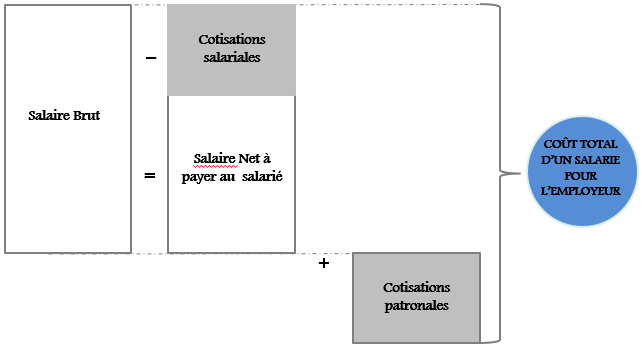
\includegraphics[scale=0.85]{images/remuneration.png}
		\caption{Schéma de synthèse sur le coût d'un salarié}
		\label{synthese-cout-salarie}
	\end{center}
\end{figure}















